\documentclass[notes]{subfiles}

\begin{document}
	\addcontentsline{toc}{section}{5.3/5.4 - The Fundamental Theorem of Calculus}
	\refstepcounter{section}
	\fancyhead[RO,LE]{\bfseries \large\nameref{cs53}} 
	\fancyhead[LO,RE]{\bfseries \currentname}
	\fancyfoot[C]{{}}
	\fancyfoot[RO,LE]{\large \thepage}	%Footer on Right \thepage is pagenumber
	\fancyfoot[LO,RE]{\large Chapter 5.3}
	
\section*{The Fundamental Theorem of Calculus}\label{cs53}
	\subsection*{Before Class}
	\subsection*{The First Fundamental Theorem}
		\begin{ex}
			The function \(f\) is given in the graph below.  Define the function \(g(x)\) by the equation \(g(x) =\ds \int_0^x f(t)\, dt\).  Find \(g(0)\), \(g(1)\), \(g(2)\), and \(g(3)\).  Then, sketch a rough graph of \(g\) on the interval \([0,3]\).
			\begin{flushleft}
				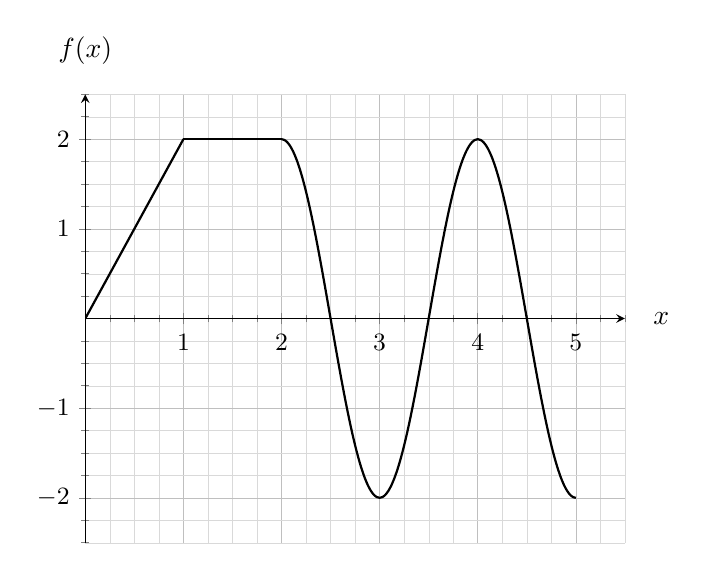
\begin{tikzpicture}
					\begin{axis}[
						grid=both,
						grid style={line width=.1pt, draw=gray!30},
						major grid style={line width=.2pt,draw=gray!50},
						every tick label/.append style={font=\small},
						axis x line = middle,
						axis y line = middle,
			    			every axis y label/.style={at={(ticklabel cs:1.15)}},
			    			%ytick = {-4, -2, -3, -1, 1, 2, 3, 4},
						y label style={at={(axis description cs:0,1.15)},anchor=north},
			    			ylabel = {$f(x)$},
		    				every axis x label/.style= {at ={(ticklabel cs:1)}},
		    				%xtick = {-4,-3,-2,-1,1,2,3,4},
		    				x label style={at={(axis description cs:1.1,.5)},anchor=east},
		    				xlabel = {$x$},
		    				xmax = 5.5, ymin = -2.5, ymax = 2.5,
		    				minor tick num = 3
					]
					
						\addplot[thick,domain = 0:1] {2*x};
						\addplot[thick,domain = 1:2] {2};
						\addplot[thick,smooth,samples=100,domain = 2:5] {2*cos((180)*(x-2))};
					\end{axis}
				\end{tikzpicture}
			\end{flushleft}
		\end{ex}
			\vs{2}
			
		\begin{thm}[The Fundamental Theorem of Calculus, Part 1 (FTC1)]
				If \(f\) is continuous on \([a,b]\), then the function \(g\) defined by\(g(x) = \ds \int_a^x f(t)\,dt\), for \(a\leq x\leq b\), is\vspace{25pt} \blank{6}\\ \\ \blank{1.5}.  Using Leibniz notation, we have\vspace{.75in}
			
		\end{thm}
			\newpage
			
		\begin{ex}
			Find the derivative of the function \(g(x) = \ds\int_0^x \sqrt{1-t^2}\,dt\).	
		\end{ex}
			\vs{1}
		\begin{ex}
			Find \(\ds\dfrac{d}{dx}\int_1^{x^2}\csc t\,dt\)
		\end{ex}
			\vs{1}
		
		\begin{ex}
			Find \(F'(x)\), if \(F(x) = \ds \int_x^0 \sqrt{1 + \sec y}\, dy\)
		\end{ex}
			\vs{1}
			\newpage

	\subsection*{Pre Class Practice}
		\begin{ex}
			Let \(g(x) = \ds \int_0^x f(t)\, dt\), where \(f\) is the function in the graph below.\\
			\includegraphics{5.3fig1}\\
			\begin{enumerate}[(a)]
				\item Evaluate \(g(0), g(1), g(2), g(3)\), and \(g(6)\).
					\vs{1}
					
				\item Where is \(g\) increasing?
					\vs{1}
					
				\item Where does \(g\) have a local max?
					\vs{1}
					
				\item Sketch a rough graph of \(g\).
					\vs{2}
					
			\end{enumerate}
		\end{ex}	
			\newpage
		
		\begin{ex}
			Find the derivative of the following functions.
			\begin{enumerate}[(a)]
				\item \(g(x) = \ds \int_2^x \sqrt{k + k^3}\, dk\)
					\vs{1}
					
				\item \(r(y) = \ds \int_y^2 t^3\cos t\, dt\)
					\vs{1}
					
				\item \(f(x) = \ds \int_0^{x^4} \tan^2t\, dt\)
					\vs{1}
			\end{enumerate}
		\end{ex}
		
		\begin{ex}
			If \(f(x) = \ds \int_0^x (1-t^2)\cos^2 t\, dt\), on what interval is \(f\) increasing?
		\end{ex}
			\vs{1}
			\newpage
			
	\subsection*{In Class}
	\subsubsection*{FTC 1 Examples}
		\begin{ex}
			Find the derivative of \(g(r) = \ds \int_r^5 (t-t^2)^8\,dt\)
		\end{ex}
			\vs{1}
			
		\begin{ex}
			Find the derivative of \(R(y) = \ds \int_{\tan y}^4 t^5e^{\cos (t+2)}\, dt\)
		\end{ex}
			\vs{1}
			
		\begin{ex}
			Find the derivative of \(y = \ds\int_0^{4x^3} \tan^2\theta\, d\theta\)
		\end{ex}
			\vs{1}
			\newpage
			
	\subsubsection*{The Second Fundamental Theorem}
		\begin{thm}[The Fundamental Theorem of Calculus, Part 2 (FTC2)]
				If \(f\) is \blank{1.5} on \([a,b]\), then\vspace{.75in}\\ where \(F\) is \blank{3}.
		\end{thm}
		\begin{ex}
			\(\ds \int_{-2}^1 x^3\,dx\)
		\end{ex}
			\vs{1}
			
		\begin{ex}
			Find the area under the curve \(y = x^2\) from 0 to 1.
		\end{ex}
			\vs{1}
			\newpage

		\begin{ex}
			Find the area under the curve \(y = \sin x\), from \(0\) to \(\dfrac{3\pi}{2}\)
		\end{ex}
			\vs{1}
			
		\begin{ex}
			Is the statement \(\ds \int_{-1}^1 \dfrac{1}{x^3}\, dx = 0\) correct?  Why or why not?
		\end{ex}
			\vs{1}
			
		\begin{ex}
			Calculate the integral \(\ds \int_1^3 (x^2+2x-4)\, dx\)
		\end{ex}
			\vs{1}
			
		\begin{ex}
			Calculate the integral \(\ds \int_0^2 \lrpar{\dfrac{4}{5}t^3-\dfrac{3}{4}t^2+\dfrac{2}{5}t}\,dt\)
		\end{ex}
			\vs{1}
			\newpage
			
		\begin{ex}
			Calculate the integral \(\ds \int_1^9 \sqrt{x}\,dx\)
		\end{ex}
			\vs{1}
	
	\subsubsection*{Applications of FTC 2}
		\begin{rmk}[Integrals of Symmetric Functions]
			For symmetric functions, we have the following properties:\\
				\begin{enumerate}[(1)]
				\setlength\itemsep{5pt}
					\item If \(f\) is continuous on \([-a,a]\) and \(f\) is even, then\vspace{.75in}
					\item If \(f\) is continuous on \([-a,a]\) and \(f\) is odd, then\vspace{.75in}
				\end{enumerate}
		\end{rmk}
		
		\begin{ex}
			Evaluate \(\ds \int_{-\pi/3}^{\pi/3} x^4\sin x\,dx\)
		\end{ex}
			\vs{1}
			
		\begin{ex}
			Compute \(\ds \int_{-\pi/4}^{\pi/4} \lrpar{x^3 + x^4 \tan x}\, dx\)
		\end{ex}
			\vs{1}
			\newpage
			
		\begin{thm}[Net Change]
			The integral of a rate of change is the net change, i.e.:
				\\ \\ \\ 
		\end{thm}
			
		\begin{rmk}[Displacement/Distance]
			When talking about physical situations, the \emph{displacement} of a particle is the
				\blank{1} \\ \\ \blank{3}, while the \emph{distance} is the 
				\blank{1.5} \\ \\ \blank{3.5}.
		\end{rmk}
			
		\begin{ex}
			A particle moves along a line so that its velocity at time \(t\) is \(v(t) = t^2-t-6\) m/s. 
			\begin{enumerate}[(a)]
				\item Find the displacement of the particle during the time period \(1\leq t\leq 4\).
					\vs{1}
					
				\item Find the distance traveled during this time period.
					\vs{1}
					
			\end{enumerate}
		\end{ex}
			\newpage
			
		\begin{ex}
			A particle moving along a line has velocity \(v(t) = t^2 -2t-3\) m/s.  Find the displacement and the total distance traveled by the particle between 1 and 4 seconds.
		\end{ex}
			\vs{1}
			
		\begin{ex}
			A honeybee population starts with 100 bees and increases at a rate of \(n'(t)\) bees per week.  What does 100 + \(\ds \int_0^{15}n'(t)\,dt\) represent?
		\end{ex}
			\vs{1}
			
	\subsubsection*{Examples}
		\begin{ex}
			Calculate the integral\(\ds \int_1^4 \dfrac{2+x^2}{\sqrt{x}}\,dx\)
		\end{ex}
			\vs{1}
			\newpage
			
		\begin{ex}
			Calculate the integral \(\ds \int_{\pi/6}^{\pi/2}\csc t\cot t\, dt\)
		\end{ex}
			\vs{1}
			
		\begin{ex}
			Calculate the integral \(\ds \int_{-1}^2 (3u-2)(u+1)\, du\)
		\end{ex}
			\vs{1}
			
		\begin{ex}
			Calculate the integral \(\ds \int_{\pi/4}^{\pi/3} \csc^2\theta\, d\theta\)
		\end{ex}
			\vs{1}
			\newpage
			
		\begin{ex}
			Calculate the integral \(\ds \int_1^{18} \sqrt{\dfrac{2}{z}}\, dz\)
		\end{ex}
			\vs{1}
			
		\begin{ex}	
			Evaluate the integral \(\ds \int_1^2 \dfrac{v^5+3v^6}{v^4}\, dv\)
		\end{ex}
			\vs{1}
			
		\begin{ex}
			Evaluate the integral \(\ds\int_0^\pi f(x)\, dx\), where \(f(x) = \begin{cases}\sin x & \text{if }0\leq x < \pi/2 \\ \cos x & \text{if }\pi/2\leq x\leq \pi \end{cases}\)
		\end{ex}
			\vs{1}
			
		\begin{ex}
			If \(f(1) = 12\), \(f'\) is continuous, and \(\ds \int_1^4 f'(x)\, dx = 17\), what is the value of \(f(4)\)?
		\end{ex}	
			\vs{1}
			\newpage
	
	\subsection*{After Class Practice}
		\begin{ex}
			Compute \(\ds \int_{-\pi/6}^{\pi/6} \dfrac{1}{\sqrt{1-x^2}}\, dx\)
		\end{ex}
			\vs{1}
			
		\begin{ex}
			If \(x\) is measured in meters and \(f(x)\) is measured in newtons, what are the units of \(\ds \int_0^{100}f(x)\,dx\)?
		\end{ex}
			\vs{1}
			
		\begin{ex}
			The acceleration function of a particle is \(a(t) = t+4\) m/s\(^2\), and its the initial velocity is 5 m/s.  Find the velocity at time \(t\), and the distance traveled between time \(t = 0\) and \(t = 5\).
		\end{ex}
			\vs{1}
			\newpage
			
		\begin{ex}
			Compute \(\ds \int_0^1 (1+r)^3\, dr\)
		\end{ex}
			\vs{1}
			
		\begin{ex}
			Find the area under the curve \(f(x) = \dfrac{x^4 + 1}{x^2}\) between 1 and 2.
		\end{ex}
			\vs{1}

		\begin{ex}
			Evaluate \(\ds \int_{-1}^1 x^{2023}\, dx\)
		\end{ex}
			\vs{1}
			
		\begin{ex}
			What does it mean for differentiation and integration to be inverse processes?
		\end{ex}
			\vs{1}
	\clearpage	
\end{document}